\documentclass[14pt]{extbook}
\usepackage{multicol, enumerate, enumitem, hyperref, color, soul, setspace, parskip, fancyhdr} %General Packages
\usepackage{amssymb, amsthm, amsmath, bbm, latexsym, units, mathtools} %Math Packages
\everymath{\displaystyle} %All math in Display Style
% Packages with additional options
\usepackage[headsep=0.5cm,headheight=12pt, left=1 in,right= 1 in,top= 1 in,bottom= 1 in]{geometry}
\usepackage[usenames,dvipsnames]{xcolor}
\usepackage{dashrule}  % Package to use the command below to create lines between items
\newcommand{\litem}[1]{\item#1\hspace*{-1cm}\rule{\textwidth}{0.4pt}}
\pagestyle{fancy}
\lhead{Makeup Progress Quiz 3}
\chead{}
\rhead{Version A}
\lfoot{4315-3397}
\cfoot{}
\rfoot{Fall 2020}
\begin{document}

\begin{enumerate}
\litem{
Choose the equation of the function graphed below.
\begin{center}
    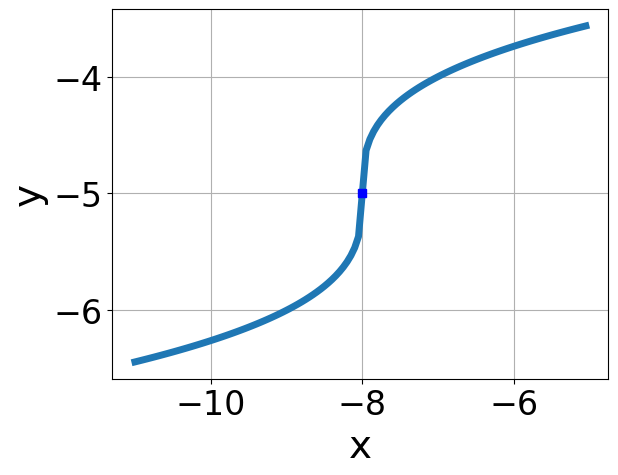
\includegraphics[width=0.5\textwidth]{../Figures/radicalGraphToEquationCopyA.png}
\end{center}
\begin{enumerate}[label=\Alph*.]
\item \( f(x) = - \sqrt[3]{x + 8} - 5 \)
\item \( f(x) = \sqrt[3]{x + 8} - 5 \)
\item \( f(x) = - \sqrt[3]{x - 8} - 5 \)
\item \( f(x) = \sqrt[3]{x - 8} - 5 \)
\item \( \text{None of the above} \)

\end{enumerate} }
\litem{
What is the domain of the function below?\[ f(x) = \sqrt[6]{5 x + 3} \]\begin{enumerate}[label=\Alph*.]
\item \( (-\infty, a], \text{where } a \in [-0.63, 1.12] \)
\item \( [a, \infty), \text{where } a \in [-7.67, -0.67] \)
\item \( (-\infty, a], \text{where } a \in [-2.04, -0.92] \)
\item \( (-\infty, \infty) \)
\item \( [a, \infty), \text{ where } a \in [-1.6, 4.4] \)

\end{enumerate} }
\litem{
Solve the radical equation below. Then, choose the interval(s) that the solution(s) belongs to.\[ \sqrt{9 x + 5} - \sqrt{-8 x - 9} = 0 \]\begin{enumerate}[label=\Alph*.]
\item \( x \in [-1.01,-0.44] \)
\item \( \text{All solutions lead to invalid or complex values in the equation.} \)
\item \( x_1 \in [-1.01, -0.44] \text{ and } x_2 \in [-3.56,2.44] \)
\item \( x \in [-0.53,0.42] \)
\item \( x_1 \in [-1.6, -1.06] \text{ and } x_2 \in [-3.56,2.44] \)

\end{enumerate} }
\litem{
Choose the graph of the equation below.\[ f(x) = \sqrt[3]{x + 6} - 7 \]\begin{enumerate}[label=\Alph*.]
\begin{multicols}{2}\item 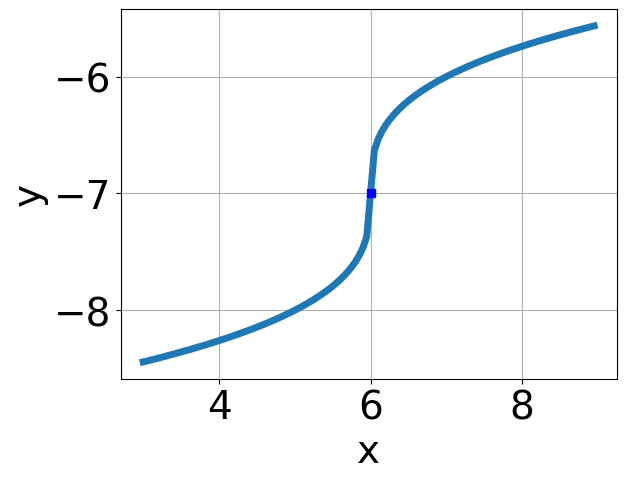
\includegraphics[width = 0.3\textwidth]{../Figures/radicalEquationToGraphAA.png}\item 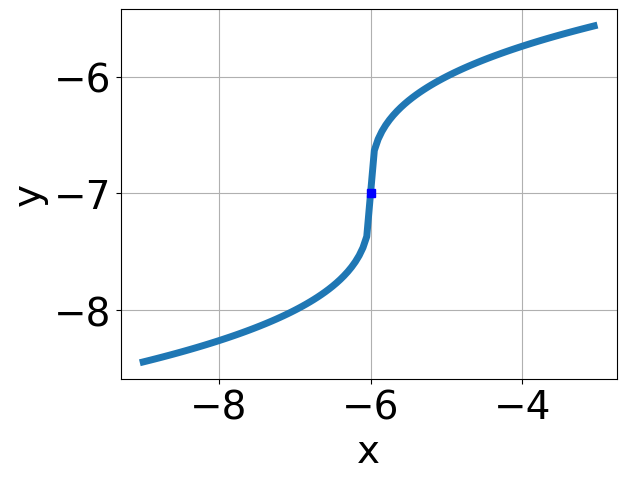
\includegraphics[width = 0.3\textwidth]{../Figures/radicalEquationToGraphBA.png}\item 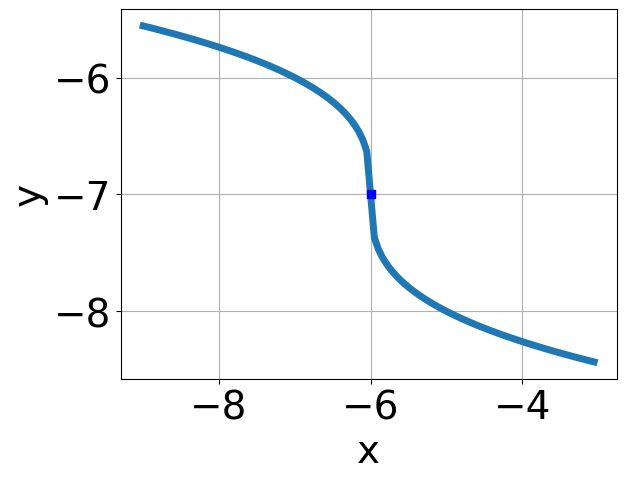
\includegraphics[width = 0.3\textwidth]{../Figures/radicalEquationToGraphCA.png}\item 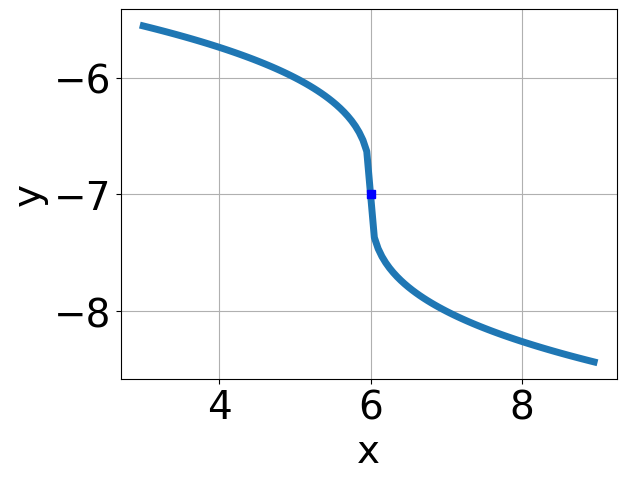
\includegraphics[width = 0.3\textwidth]{../Figures/radicalEquationToGraphDA.png}\end{multicols}\item None of the above.
\end{enumerate} }
\litem{
What is the domain of the function below?\[ f(x) = \sqrt[5]{-6 x + 7} \]\begin{enumerate}[label=\Alph*.]
\item \( \text{The domain is } [a, \infty), \text{   where } a \in [-1.3, 0.9] \)
\item \( (-\infty, \infty) \)
\item \( \text{The domain is } (-\infty, a], \text{   where } a \in [1.04, 1.66] \)
\item \( \text{The domain is } (-\infty, a], \text{   where } a \in [0.33, 1.07] \)
\item \( \text{The domain is } [a, \infty), \text{   where } a \in [1.1, 1.7] \)

\end{enumerate} }
\litem{
Choose the graph of the equation below.\[ f(x) = \sqrt[3]{x + 14} + 6 \]\begin{enumerate}[label=\Alph*.]
\begin{multicols}{2}\item 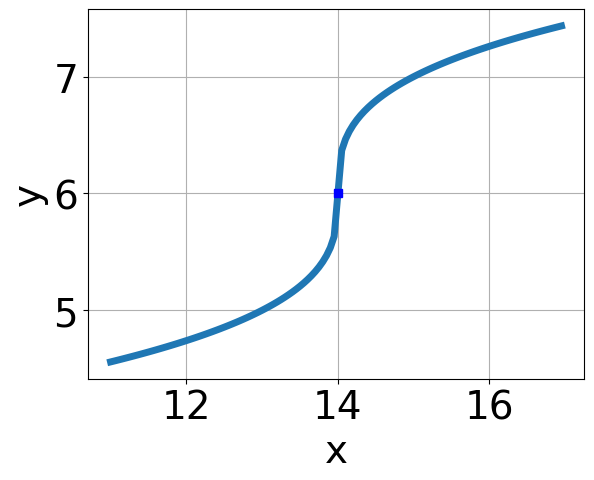
\includegraphics[width = 0.3\textwidth]{../Figures/radicalEquationToGraphCopyAA.png}\item 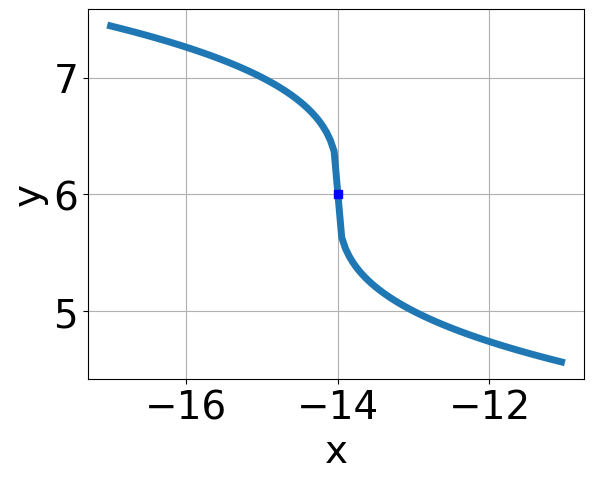
\includegraphics[width = 0.3\textwidth]{../Figures/radicalEquationToGraphCopyBA.png}\item 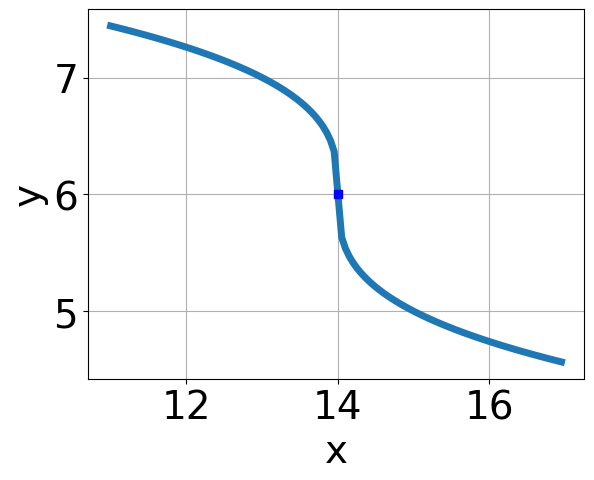
\includegraphics[width = 0.3\textwidth]{../Figures/radicalEquationToGraphCopyCA.png}\item 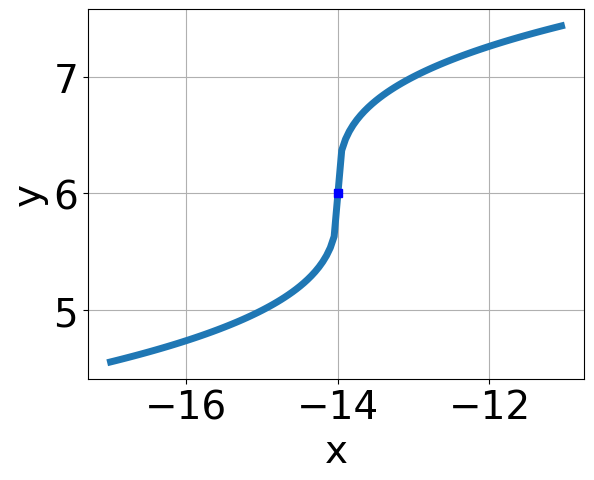
\includegraphics[width = 0.3\textwidth]{../Figures/radicalEquationToGraphCopyDA.png}\end{multicols}\item None of the above.
\end{enumerate} }
\litem{
Solve the radical equation below. Then, choose the interval(s) that the solution(s) belongs to.\[ \sqrt{36 x^2 + 63} - \sqrt{99 x} = 0 \]\begin{enumerate}[label=\Alph*.]
\item \( x_1 \in [0.45, 1.19] \text{ and } x_2 \in [1.75,4.75] \)
\item \( x_1 \in [-1.78, -1.14] \text{ and } x_2 \in [-4,1] \)
\item \( x \in [1.16,1.94] \)
\item \( \text{All solutions lead to invalid or complex values in the equation.} \)
\item \( x \in [0.45,1.19] \)

\end{enumerate} }
\litem{
Solve the radical equation below. Then, choose the interval(s) that the solution(s) belongs to.\[ \sqrt{-24 x^2 + 45} - \sqrt{-57 x} = 0 \]\begin{enumerate}[label=\Alph*.]
\item \( x_1 \in [0, 1.7] \text{ and } x_2 \in [1,5] \)
\item \( \text{All solutions lead to invalid or complex values in the equation.} \)
\item \( x_1 \in [-1.5, -0.5] \text{ and } x_2 \in [1,5] \)
\item \( x \in [2.3,3.4] \)
\item \( x \in [-1.5,-0.5] \)

\end{enumerate} }
\litem{
Solve the radical equation below. Then, choose the interval(s) that the solution(s) belongs to.\[ \sqrt{5 x - 2} - \sqrt{-4 x + 6} = 0 \]\begin{enumerate}[label=\Alph*.]
\item \( x_1 \in [-0.11, 0.61] \text{ and } x_2 \in [0.45,1.22] \)
\item \( x \in [0.73,1.17] \)
\item \( x_1 \in [-0.11, 0.61] \text{ and } x_2 \in [1.09,1.53] \)
\item \( x \in [-0.82,-0.25] \)
\item \( \text{All solutions lead to invalid or complex values in the equation.} \)

\end{enumerate} }
\litem{
Choose the equation of the function graphed below.
\begin{center}
    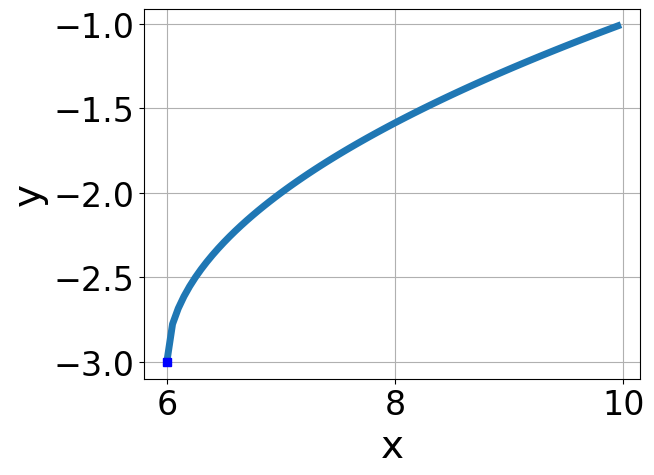
\includegraphics[width=0.5\textwidth]{../Figures/radicalGraphToEquationA.png}
\end{center}
\begin{enumerate}[label=\Alph*.]
\item \( f(x) = - \sqrt{x - 6} - 3 \)
\item \( f(x) = \sqrt{x - 6} - 3 \)
\item \( f(x) = \sqrt{x + 6} - 3 \)
\item \( f(x) = - \sqrt{x + 6} - 3 \)
\item \( \text{None of the above} \)

\end{enumerate} }
\end{enumerate}

\end{document}